\documentclass{article}
\usepackage{graphicx,hyperref}
\usepackage{amsmath,amsfonts,amsthm,fullpage}
\usepackage{algorithm}
\usepackage{algorithmic}
\usepackage{listings}
\usepackage{mathtools}
\usepackage{caption}
\usepackage{subfig}
\graphicspath{ {figures/} }
\usepackage{cleveref}
\usepackage{array}
\usepackage[many]{tcolorbox}    % for COLORED BOXES (tikz and xcolor included)\usepackage[many]{tcolorbox} 
% for COLORED BOXES (tikz and xcolor included)
\usepackage{setspace}               % for LINE SPACING
\usepackage{multicol}               % for MULTICOLUMNS
\usepackage{enumitem}
\usepackage[english]{babel} % To obtain English text with the blindtext package
\usepackage{blindtext}
\usepackage{biblatex} %Imports biblatex package
\addbibresource{ISyE6740Projecttemplate.bib} %Import the bibliography file


% You can copy any following box you like to your code.
\newtcolorbox{boxA}{
	fontupper = \bf,
	boxrule = 1.5pt,
	colframe = black % frame color
}

\usepackage[margin=1in]{geometry}

\begin{document}
%	\begin{titlepage}
%		\clearpage\thispagestyle{empty}
%		\centering
%		\vspace{1cm}
%		
%		\rule{\linewidth}{1mm} \\[0.5cm]
%		{ \Large \bfseries ISYE 7406 - Spring 2023\\[0.2cm]
%			Proposal}\\[0.5cm]
%		\rule{\linewidth}{1mm} \\[1cm]
%		
%		\begin{tabular}{l p{5cm}}
%			\textbf{Team Member Names:} Andrew Bartels&   \\
%			\textbf{Project Title:} Lid Driven Cavity Flow: 
%			A Physics Informed Neural Network Approach vs. \\
%			 Traditional Statistical Models &  \\
%			
%		\end{tabular} 
%	\end{titlepage}
	
	% make a table of contents from the sections
%	\tableofcontents
%	\clearpage
%	\thispagestyle{empty}
%	\listoffigures
%	% \listoftables % if we have tables?
%	\newpage
%	\pagenumbering{arabic}

	\title{ISYE 7406 - Spring 2023 Project Proposal \\
	 Lid Driven Cavity Flow: 
				A Physics Informed Neural Network Approach vs. \\
				 Traditional Statistical Model}
	
	\maketitle
	
	Project Member(s): Andrew Bartels
	
	\section{Problem Description}
	
	\indent Computational fluid dynamics (CFD) is the process of mathematically modeling a physical phenomenon involving fluid flow and solving it numerically using computers. From winning race cars to commercial aircraft that people fly in every day, CFD is a fundamental process in the pipeline from idea to design, while saving millions in costs. Rather than building multiple versions and prototyping (which is exceedingly expensive), engineers today will simply run a series of models to find the best design and then iterate this into a final product. The main issue with this is depending on the detail and length of the simulation, even the most basic simulations will either cost many thousands of dollars on a high performance computing (HPC) cluster, or take a very long time to run on a standard desktop or laptop (usually in terms of weeks to months). \\
%	
%	\begin{figure}[h]
%		\centering
%		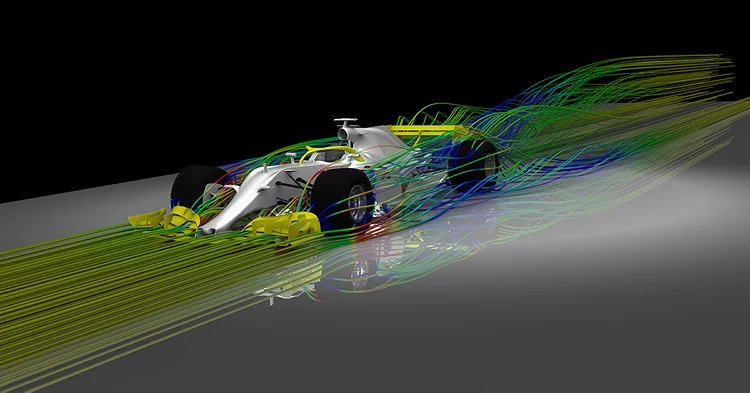
\includegraphics[scale=0.4]{./images/cfd.jpg}
%		\caption{A picture of CFD model \cite{ANSYS.com}}
%		\label{fig:CFD_Image}
%	\end{figure}
%	
	In the separate field of machine learning, neural networks and other non-explicitly programmed algorithms are estimated to be an industry in the billions. This has led to an explosion in interest and growth into the field, with researchers and scientists applying neural networks to more applications than just image identification. While these statisical models can capture nonlinear effects very well, they often require hundreds or millions of examples to fit a model, where generalization of new data is not always guaranteed. Conversely, in CFD, data is often measured in terms of gigabytes to petabytes, so sifting through this data for meaning or trying to feed more than a few examples to a neural network can be extremely prohibitive (time and cost). This leads to the introduction of physics informed neural networks (PINNs). This is where the loss function of the optimization is substituted for a part of physics (in this study, the continuity equation), in order for the model to adhere to physics better. This has led to models that adhere to physics applications much better with less data, converge to a solution faster, and put "guard rails" on models that attempt to predict vastly different phenomena that might be practical. Furthermore, traditional statistical models that are feasibly equipped to predict non-linear events will also be studied (such as SVM kernels, KNN, and others from this data mining class).
	
	\pagebreak
	
	\subsection{Problem Setup}
	
	In this study a classic fluid mechanics problem will be observed with an application of PINNs and other statistical models, specifically the Lid-driven cavity flow problem (or sometime referenced as the driven cavity flow problem). This is a 2 dimensional application of the Navier-Stokes equation with the simplifications of being in 2 dimensions, steady-state, incompressible fluid flow, at lower Reynolds number ($\le 2000$). This is a well studied test case with many permutations such as nonlinear gridding, spectral methods and different optimization algorithms for faster convergence, however this is all outside the scope of this study. The algorithm used as baseline is the \href{https://en.wikipedia.org/wiki/SIMPLE_algorithm}{SIMPLE} (Semi-Implicit Method for Pressure Linked Equations) algorithm. For the baseline examples to reproduce Reynolds numbers between roughly 300-1,900. A PINN will then be trained with the same grid size and continuity equation as the optimization function. A comparison between the baseline and machine learned approaches will then be quantitatively compared. This will then give a further insight into the usefulness of PINNs (and versus other traditional algorithms from this class), and how generalizable something like this could become in the future development in this field of study.
	
	\begin{figure}[ht!]
		\centering
		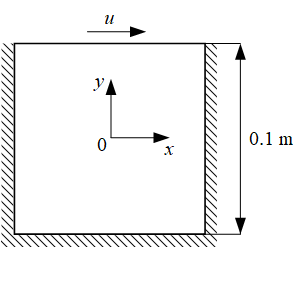
\includegraphics[scale=0.7]{./images/ldc.png}
		\caption{Open Lidded Cavity Flow Free Body Diagram}
		\label{fig:OLC}
	\end{figure}
	
	\subsection{Data}
	
	For this project proposal, the data will be generated using \textcolor{blue}{\href{https://www.openfoam.com/documentation/tutorial-guide/2-incompressible-flow/2.1-lid-driven-cavity-flowURL}{openFOAM}} which will need conversion and reading from the open source openFOAM data format to something python readable by PyTorch and scikit learn. \\
	
	\noindent The other possible approach for generating the data will be \textcolor{blue}{\href{https://github.com/gauravsdeshmukh/FlowPy}{FlowPy}} (in pure python)
	
	\subsection{Scientific Research Questions}
	
	The overall theme of these questions are if statistical models could help traditional computational methods be either faster (skip the long computational times via prediction) or produce results similar to empirical/computational methods for extrapolation (data from slower speed flows, accurately predict higher flow problems)
	
	\begin{enumerate}
		\item Can Physics Informed Neural Network (PINNs) be properly taught to generalize a canonical non-linear problem in fluid mechanics.
		\item Would more traditional algorithms better generalize to non-linear physics effects
		\item Do any statistical models predict or produce accurate results compared to expensive computational methods
		\item Are there any features that can be mined from the data or derived that can better produce more accurate prediction results 
	\end{enumerate}
	
%	\subsection{Computational Fluids Overview}
%	
%	Computational fluid dynamics (CFD) is the science of predicting fluid flow, heat transfer, mass transfer, chemical reactions, and
%	related phenomena by solving the mathematical equations which govern these processes using a numerical process.\cite{Bakker}
%	CFD is one of the most impactful uses of physics and computers in current century. Since the creation of the Navier-Stokes (N-S) equations in the 1820s, scientists, physicists, and engineers have tried to create faster and more efficient ways to model fluid flows to make more informed decisions and designs \cite{Bakker}. Depending on the different assumptions one might make when creating a fluid simulation in a computer, the time it takes to calculate the final simulation or time series of a fluid flow can vary greatly from a matter of seconds for a RANs (Reynolds Averaged N-S) simulation, all the way to Direct Numerical Simulation (DNS) where turbulent features are fully resolved with an extremely high resolution model even for simple cases. For better reference see \ref{fig:complex} to visually show how different fluid models resolve energy dissipation (viscosity) throughout the simulation.
%	
%	% maybe put CFD workflow and talk about how it could be replaced helped my ML applications
%	
%	\begin{figure}[ht!]
%		\centering
%		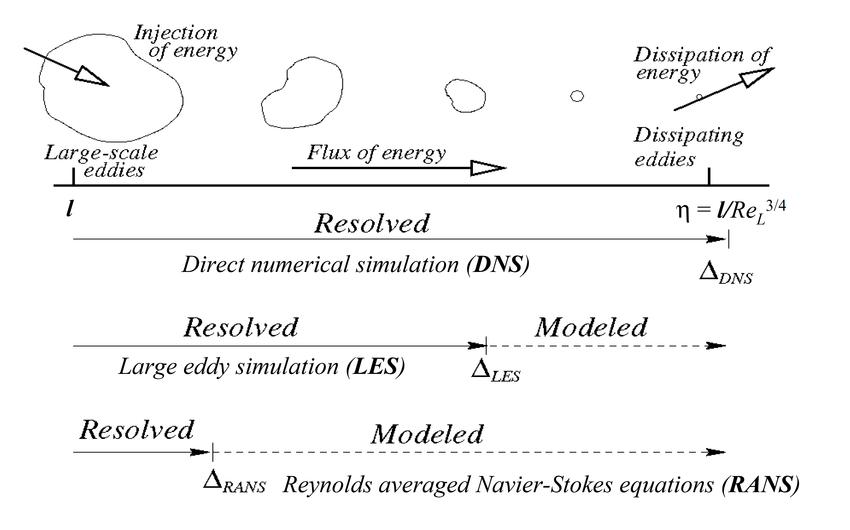
\includegraphics[scale=0.4]{./images/complex.png}
%		%		https://www.researchgate.net/figure/Schematic-representation-of-the-concept-of-DNS-LES-and-RANS-models-to-energy-cascade_fig1_305496320 
%		\caption{A picture of CFD model complexity versus reality}
%		\label{fig:complex}
%	\end{figure}
%	
%	\pagebreak
%	\subsection{Physics Informed Neural Networks (PINNs) Overview} \label{PINN}		
%	
%	\begin{figure}[ht!]
%		\centering
%		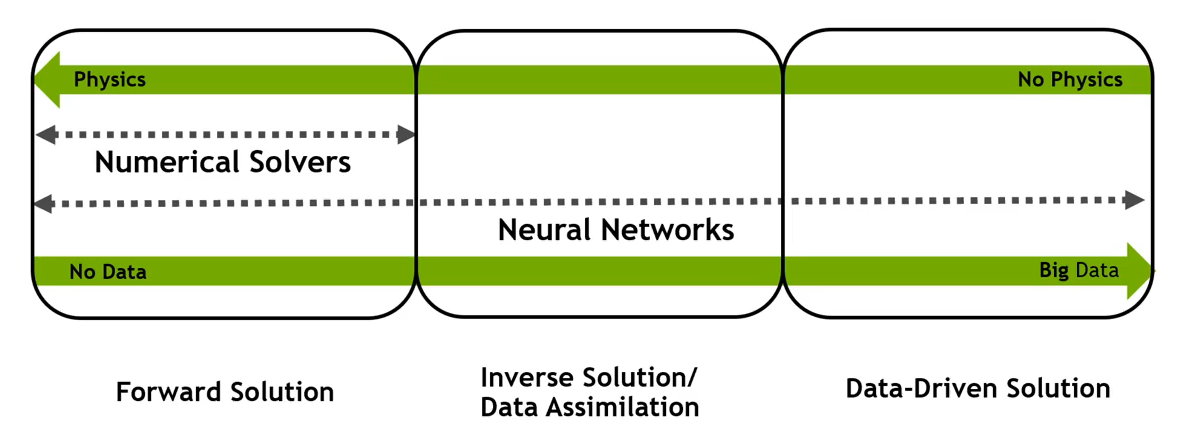
\includegraphics[scale=0.4]{./images/ai_in_computational_sciences_spectrum.png}
%		\caption{A picture of PINN spectrum from Nvidia $Modulus^{\copyright}$ \cite{NVIDIA}}
%		\label{fig:CFD_Image}
%		\label{fig:PINN_spectrum}
%	\end{figure}
%	
%	% 	https://en.wikipedia.org/wiki/History_of_artificial_neural_networks
%	%   https://towardsdatascience.com/a-concise-history-of-neural-networks-2070655d3fec
%	%   basically just summarize this with some research paper citation, and this one
%	%   
%	
%	Physics-informed machine learning debuted in the 1990s, with a few scattered publications throughout the decade, but did not gain traction until around 2010 when there was a resurgence in machine learning. The year 2011 introduced Google Brain, a cutting-edge platform capable of discovering and categorizing relatively simple objects (with a highlighted capability to identify cats.)[10] Another machine learning milestone was achieved in 2014 with Facebook’s DeepFace Algorithm being able to detect whether two faces in unfamiliar photos were of the same person with 97.25\% accuracy, a metric that effectively rivaled human perception.[10] By the late 2010s, increases in computational power had become more easily accessible to the average researcher, and thus, applications of machine learning to other scientific fields became increasingly prevalent. 
%	
%	In the past few years, physics-informed neural networks (also known as PINNs) have allowed scientists to tackle problems that were previously out of reach. It is important to recognize that PINNs differ from traditional neural networks in that PINNs use constraints bound by physical laws or equations. Instead of feeding random data points to the neural network, the input data is purposefully constrained according to the physical model that the data should satisfy [10]. For example, in 2020 within the field of drug discovery, a PINN-based model was built that embedded prior knowledge about molecular structure in a neural network to facilitate the identification of molecular water configurations with preferrable properties. [10] In particular, however, PINNs have had a significant impact within the field of computational fluid dynamics for their ability to tackle traditionally expensive problems. \cite{PINN_History}
%	
%	Previous papers have by Raissi’s group have demonstrated how PINNs can seamlessly integrate multifidelity/multi-modality experimental data with the various Navier–Stokes formulations for incompressible flows \cite{DBLP:journals/corr/abs-1711-10561,DBLP:journals/corr/abs-1711-10566} as well as compressible flows \cite{physics-informed-machine-learning} and biomedical fluid flows. Additionally, Raissi’s group have introduced hidden physics models, which are essentially data-efficient learning machines capable of leveraging the underlying laws of physics, expressed by time dependent and nonlinear partial differential equations, to extract patterns from high-dimensional data generated from experiments. [10]
%	This study builds upon Raissi’s framework, and in order to reproduce results, we have substituted programming packages when necessary (i.e. using pytorch in lieu of tensorflow.) 
%	
%	\subsection{Traditional Statistical Models} \label{Traditional-stats-models}
%	
%	
%	
%	\section{Theory Overview} \label{theory}
%	
%	The general idea of this section is to give a general overview of the Navier-Stokes equations in a more applied sense, so a reader could have more context while not requiring an intimate knowledge of fluid mechanics to effectively analyze the results of the study. These equations are named after Claude-Louis Navier (1785-1836) and George Gabriel Stokes (1819-1903). The Navier-Stokes equations consist of a time-dependent continuity equation for conservation of mass, three time-dependent conservation of momentum equations, and time-dependent conservation of energy equation. There are four independent variables in the problem, the x, y, and z spatial coordinates of some domain and the time t.\cite{NASA} They are second-order nonlinear partial differential equations, and in multiple simplified forms have known analytical solutions. \textit{\textbf{In other words, the N-S equations describe (fully) how the velocity, pressure, temperature, and density of a moving fluid are related.}} An analytical solution of the full form would win someone a million dollars from the 	\href{https://www.claymath.org/millennium-problems/navier%E2%80%93stokes-equationURL}{Millenium prize series}. \\
%	
%	% from https://www.nuclear-power.com/nuclear-engineering/fluid-dynamics/navier-stokes-equations/
%	
%	\noindent To get started the "general" form of the N-S equations (in the convective form) will be presented:
%	
%	\begin{boxA}
%		Continuity Equation: 
%		\begin{equation}
%			\nabla \cdot \vec{V} = 0
%		\end{equation}
%		Momentum Equation(s):
%		\begin{equation}
%			\rho \frac{D \vec{V}}{Dt} = -\nabla p + \rho \vec{g} + \mu \nabla^2 \vec{V}
%		\end{equation}
%		
%	\end{boxA}
%	% momentum explanation
%	% * {{math|{{sfrac|''D''|''Dt''}}}} is the [[material derivative]], defined as {{math|{{sfrac|∂|∂''t''}} + '''u''' ⋅ ∇}},
%	% * {{math|''ρ''}} is the density,
%	% * {{math|'''u'''}} is the flow velocity,
%	% * {{math|∇ ⋅}} is the [[divergence]],
%	% * {{math|''p''}} is the [[pressure]],
%	% * {{math|''t''}} is [[time]],
%	% * {{math|'''τ'''}} is the [[Deviatoric stress|deviatoric stress tensor]], which has order 2,
%	% * {{math|'''g'''}} represents [[body force|body acceleration]]s acting on the continuum, for example [[gravity]], [[Fictitious force|inertial accelerations]], [[Coulomb's law|electrostatic accelerations]], and so on,
%	
%	% 	continuity explanation 
%	%     * {{math|''ρ''}} is fluid [[density]],
%	%     * {{math|''t''}} is time,
%	%     * {{math|'''u'''}} is the [[flow velocity]] [[vector field]].
%	
%	This is the most concise full form (no assumptions) of the N-S equation, and the differential form with assumptions will be seen in the Methodology [\ref{methodology}] section. In general terms, the continuity equation is a time-dependent way to account for the conservation of mass (back to Newton's laws of physics) such that no mass is created or destroyed in the area of observation these equations are being applied. The Momentum equations are time-dependent conservation of energy (ensuring no energy is created nor destroyed). Below is an  illustration for the explanation of each term in the equation.
%	
%	\begin{figure}[htb]
%		\centering
%		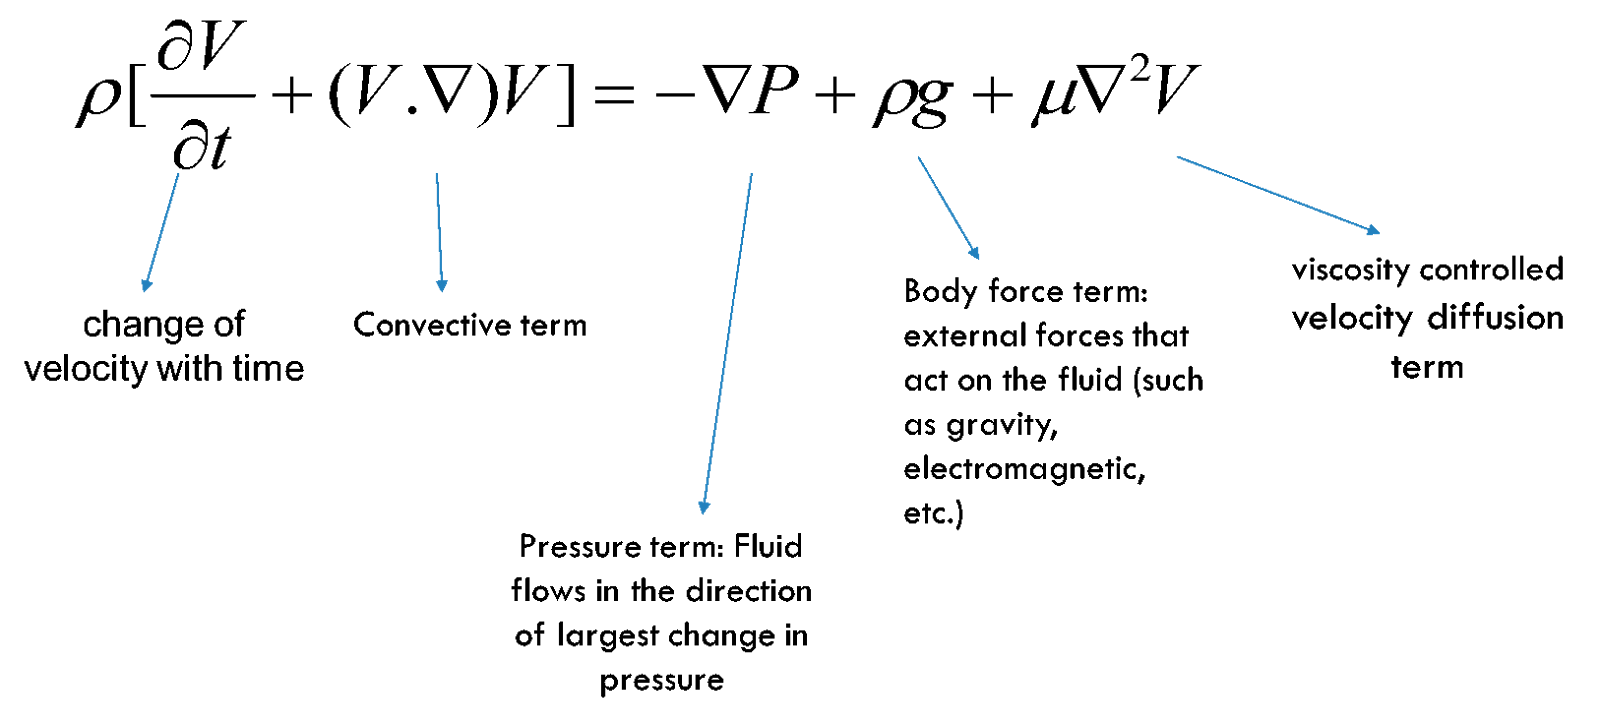
\includegraphics[scale=0.25]{./images/f.png}\label{fig:ns_ref}
%		\caption{Navier-Stokes Explained\cite{sim_world_2014} }
%	\end{figure}
%	
%	
%	It is worth noting the "Convective Term" is simply a physical process that occurs in a flow of gas in which some property is transported by the ordered motion of the flow.\cite{NASA}
%	Additionally, the "velocity diffusion" term is a physical process that occurs in a flow of gas in which some property is transported by the random motion of the molecules of the gas. Diffusion is related to the stress tensor and to the viscosity of the gas. Turbulence, and the generation of boundary layers, are the result of diffusion in the flow.
%	
%	Moreover, to solve a flow problem, you have to solve all five equations simultaneously; that is why we call this a \textit{\textbf{coupled}} system of equations. There are actually some other equation that are required to solve this system. We only show five equations for six unknowns. An equation of state relates the pressure, temperature, and density of the gas. And we need to specify all of the terms of the stress tensor. In CFD the stress tensor terms are often approximated by a turbulence model. \cite{NASA}
%	
%	\section{Methodology\cite{Barba2019}}\label{methodology}
%	
%	This study will implement the Cavity Flow with Navier–Stokes problem using a system of three differential equations. The first two equations are for the velocity components $u,v$. The third equation is for pressure $p$. Then using neural networks, the optimization function of a network will be replaced with a loss function form of the continuity equation in attempt to create a computationally efficient and faster model, while fitting a model that adheres to physics. The derivation below is for an open lidded cavity problem where the assumptions are:
%	
%	\begin{enumerate}
%		\item Two Dimensional (x and y)
%		\item Incompressible ($\rho$ is a constant number)
%		\item Laminar, turbulence is minimal, the mean Reynolds number $\le 2000$
%	\end{enumerate} 
%	
%	\noindent Now starting with the fundamental equations for this problem:\\
%	
%	\begin{align*}
%		\frac{\partial u}{\partial t}+u\frac{\partial u}{\partial x}+v\frac{\partial u}{\partial y} = -\frac{1}{\rho}\frac{\partial p}{\partial x}+\nu \left(\frac{\partial^2 u}{\partial x^2}+\frac{\partial^2 u}{\partial y^2} \right)  \\ 
%		\frac{\partial v}{\partial t}+u\frac{\partial v}{\partial x}+v\frac{\partial v}{\partial y} = -\frac{1}{\rho}\frac{\partial p}{\partial y}+\nu\left(\frac{\partial^2 v}{\partial x^2}+\frac{\partial^2 v}{\partial y^2}\right) \\
%		\frac{\partial^2 p}{\partial x^2}+\frac{\partial^2 p}{\partial y^2} = -\rho\left(\frac{\partial u}{\partial x}\frac{\partial u}{\partial x}+2\frac{\partial u}{\partial y}\frac{\partial v}{\partial x}+\frac{\partial v}{\partial y}\frac{\partial v}{\partial y} \right)     
%	\end{align*}
%	
%	
%	\noindent Each of these equations will then be Discretized as follows: \\
%	
%	\noindent Discretization of the $u$-momentum equation:
%	
%	\begin{multline}
%		\frac{u_{i,j}^{n+1}-u_{i,j}^{n}}{\Delta t}+u_{i,j}^{n}\frac{u_{i,j}^{n}-u_{i-1,j}^{n}}{\Delta x}+v_{i,j}^{n}\frac{u_{i,j}^{n}-u_{i,j-1}^{n}}{\Delta y} = \\ 
%		\qquad -\frac{1}{\rho}\frac{p_{i+1,j}^{n}-p_{i-1,j}^{n}}{2\Delta x}+\nu \left(\frac{u_{i+1,j}^{n}-2u_{i,j}^{n}+u_{i-1,j}^{n}}{\Delta  x^2}+\frac{u_{i,j+1}^{n}-2u_{i,j}^{n}+u_{i,j-1}^{n}}{\Delta y^2}\right)
%	\end{multline}
%	
%	\noindent Discretization of the $v$-momentum equation:
%	
%	\begin{multline}
%		\frac{v_{i,j}^{n+1}-v_{i,j}^{n}}{\Delta t}+u_{i,j}^{n}\frac{v_{i,j}^{n}-v_{i-1,j}^{n}}{\Delta x}+v_{i,j}^{n}\frac{v_{i,j}^{n}-v_{i,j-1}^{n}}{\Delta y} = \\
%		\qquad -\frac{1}{\rho}\frac{p_{i,j+1}^{n}-p_{i,j-1}^{n}}{2\Delta y} 
%		+\nu\left(\frac{v_{i+1,j}^{n}-2v_{i,j}^{n}+v_{i-1,j}^{n}}{\Delta x^2}+\frac{v_{i,j+1}^{n}-2v_{i,j}^{n}+v_{i,j-1}^{n}}{\Delta y^2}\right)
%	\end{multline}
%	
%	\noindent Discretization of the pressure-Poisson equation:
%	
%	\begin{equation}
%		\begin{aligned}
%			\frac{p_{i+1,j}^{n}-2p_{i,j}^{n}+p_{i-1,j}^{n}}{\Delta x^2}+\frac{p_{i,j+1}^{n}-2p_{i,j}^{n}+p_{i,j-1}^{n}}{\Delta y^2} & = \\
%			& \qquad \rho \biggr[ \frac{1}{\Delta t}\left(\frac{u_{i+1,j}-u_{i-1,j}}{2\Delta x}+\frac{v_{i,j+1}-v_{i,j-1}}{2\Delta y}\right) \\
%			& -\frac{u_{i+1,j}-u_{i-1,j}}{2\Delta x}\frac{u_{i+1,j}-u_{i-1,j}}{2\Delta x} \\ 
%			& - 2\frac{u_{i,j+1}-u_{i,j-1}}{2\Delta y}\frac{v_{i+1,j}-v_{i-1,j}}{2\Delta x} \\
%			& - \frac{v_{i,j+1}-v_{i,j-1}}{2\Delta y}\frac{v_{i,j+1}-v_{i,j-1}}{2\Delta y} \biggr]
%		\end{aligned}
%	\end{equation}
%	
%	\noindent The discretized equations can once again be rearranged to convey how iterations will proceed in the code.\\
%	
%	\noindent  The momentum equation in the $u$ direction:
%	
%	\begin{equation}
%		\begin{aligned}
%			u_{i,j}^{n+1} & = \\
%			& u_{i,j}^{n} - u_{i,j}^{n} \frac{\Delta t}{\Delta x} \left(u_{i,j}^{n}-u_{i-1,j}^{n}\right) - v_{i,j}^{n} \frac{\Delta t}{\Delta y} \left(u_{i,j}^{n}-u_{i,j-1}^{n}\right) \\
%			& - \frac{\Delta t}{\rho 2\Delta x} \left(p_{i+1,j}^{n}-p_{i-1,j}^{n}\right) \\
%			& + \nu \left(\frac{\Delta t}{\Delta x^2} \left(u_{i+1,j}^{n}-2u_{i,j}^{n}+u_{i-1,j}^{n}\right) + \frac{\Delta t}{\Delta y^2} \left(u_{i,j+1}^{n}-2u_{i,j}^{n}+u_{i,j-1}^{n}\right)\right)
%		\end{aligned}
%	\end{equation}
%	
%	
%	\noindent The momentum equation in the $v$ direction:
%	
%	\begin{equation}
%		\begin{aligned}
%			v_{i,j}^{n+1} &= \\
%			& v_{i,j}^{n} - u_{i,j}^{n} \frac{\Delta t}{\Delta x} \left(v_{i,j}^{n}-v_{i-1,j}^{n}\right) - v_{i,j}^{n} \frac{\Delta t}{\Delta y} \left(v_{i,j}^{n}-v_{i,j-1}^{n})\right) \\
%			& - \frac{\Delta t}{\rho 2\Delta y} \left(p_{i,j+1}^{n}-p_{i,j-1}^{n}\right) \\
%			& + \nu \left(\frac{\Delta t}{\Delta x^2} \left(v_{i+1,j}^{n}-2v_{i,j}^{n}+v_{i-1,j}^{n}\right) + \frac{\Delta t}{\Delta y^2} \left(v_{i,j+1}^{n}-2v_{i,j}^{n}+v_{i,j-1}^{n}\right)\right)
%		\end{aligned}
%	\end{equation}
%	
%	
%	\noindent  Rearrangement of the pressure-Poisson equation:
%	
%	\begin{equation}
%		\begin{aligned}
%			p_{i,j}^{n} & =  \\
%			& \frac{\left(p_{i+1,j}^{n}+p_{i-1,j}^{n}\right) \Delta y^2 + \left(p_{i,j+1}^{n}+p_{i,j-1}^{n}\right) \Delta x^2}{2\left(\Delta x^2+\Delta y^2\right)} \\
%			& -\frac{\rho\Delta x^2\Delta y^2}{2\left(\Delta x^2+\Delta y^2\right)} \\
%			& \times \biggr[\frac{1}{\Delta t}\left(\frac{u_{i+1,j}-u_{i-1,j}}{2\Delta x}+\frac{v_{i,j+1}-v_{i,j-1}}{2\Delta y}\right)  -\frac{u_{i+1,j}-u_{i-1,j}}{2\Delta x}\frac{u_{i+1,j}-u_{i-1,j}}{2\Delta x} \\ 
%			& - 2\frac{u_{i,j+1}-u_{i,j-1}}{2\Delta y}\frac{v_{i+1,j}-v_{i-1,j}}{2\Delta x}- \frac{v_{i,j+1}-v_{i,j-1}}{2\Delta y}\frac{v_{i,j+1}-v_{i,j-1}}{2\Delta y}\biggr]
%		\end{aligned}
%	\end{equation}
%	\linebreak
%	\linebreak
%	
%	\begin{boxA}
%		This study will have the initial conditions $u, v, p = 0$ everywhere. \\ 
%		\\
%		The boundary conditions will be: 
%		\begin{itemize}
%			\item $u=1$ at $y=2$ (the "lid");
%			\item $u, v=0$ on the other boundaries;
%			\item $\frac{\partial p}{\partial y}=0$ at $y=0$;
%			\item $p=0$ at $y=2$
%			\item $\frac{\partial p}{\partial x}=0$ at $x=0,2$
%		\end{itemize}
%	\end{boxA}
%	
%	\subsection{PINN Optimization \& Neural Network Layout}
%	
%	IN PROGRESS!!!!!
%	
%	\noindent Lastly, this section will enumerate the optimization and loss function theory that makes a neural network a "PINN" (see PINN Overview Section \ref{PINN}). The following methodology is emulated from \citeauthor{DBLP:journals/corr/abs-1711-10566}\cite{DBLP:journals/corr/abs-1711-10566}(with small alterations). To begin, this form of the Navier-Stokes takes a 2D equation  with while studying percentage of noise, however, this noise input was not implemented in this study. The $\lambda$ term below was still used to optimize the model to
%	it's final solution. Additionally, the subscript denotes the derivative w.r.t. the variable, and the double subscript the second derivative.\\
%	
%	\begin{equation}
%		\begin{aligned}
%			u_{t} + \lambda_{1} (u u_{x} + v u_{x}) & = - p_{x} + \lambda_{2}(u_{xx} + u_{yy}) \\
%			v_{t} + \lambda_{1} (u v_{x} + v v_{y}) & = - p_{y} + \lambda_{2}(u_{xx} + u_{yy}) 
%		\end{aligned}
%	\end{equation}
%	
%	\noindent This is the Navier stokes simplified in two dimensions where $ u(t,x,y) $ denotes the $x$-component of the velocity field, $ v(t,x,y) $ the $y$-component, and finally $ p(t,x,y) $ being the pressure. Additionally $\lambda = (\lambda_{1}, \lambda_{2})$ are the unknowns of the function. Invoking inviscid fluid theory a typical assumptions are the following:
%	
%	
%	\begin{align}
%		u = \psi_{y} && v = -\psi_{x}
%	\end{align}
%	
%	\noindent To invoke the continuity  the following was used, where this study added in an additional latent term of the Reynolds number ($Re$, in attempt to embed additional characteristics of the fluid flow in the cavity):
%	
%	\begin{equation}
%		\{t^i, x^i, y^i, u^i, v^i, Re^i\}^{N}_{i=1}
%	\end{equation}
%	
%	\noindent furthermore, \citeauthor{DBLP:journals/corr/abs-1711-10566} used the following functions to define the approximation $\left[ \psi(t,x,y), p(t,x,y)\right]$
%	
%	\begin{equation}
%		\begin{aligned}
%			f(t,x,y) & \coloneqq u_t + \lambda_1 ( u u_x + v u_y) + p_x - \lambda_{2}(u_{xx} + u_{yy}) \\ 
%			g(t,x,y) & \coloneqq v_t + \lambda_1 ( u v_x + v v_y) + p_x - \lambda_{2}(v_{xx} + v_{yy})
%		\end{aligned}
%	\end{equation}
%	
%	\noindent Therefore the functions above are now the critical optimization parameter for the model to tune the network weights. While the mean squared error loss is now defined as:
%	
%	\begin{align}
%		MSE & \coloneqq \frac{1}{N} \sum_{i=1}^{N} ( |u(t^i,x^i,y^i) - u^i |^2 + | v(t^i,x^i,y^i) - v^i |^2)\\
%		& + \frac{1}{N} \sum_{i=1}^{N} ( |f(t^i,x^i,y^i)|^2 + | g(t^i,x^i,y^i)|^2)
%	\end{align}
%	
%	\noindent Lastly, the network used was just a simple array of fully connected layers with the input being [batch size x 4 x grid size\textsuperscript{2}] where for this study a grid of 151x151 in the x and y direction was used for the truthly data of the \textit{\underline{\href{https://github.com/gauravsdeshmukh/FlowPy}{FlowPy} }} python model. This python code for computing the traditional lid driven cavity solution was fundamental.\textsuperscript{\cite{Barba2019, FlowPy}} \\
%	
%	\noindent As seen in the table below, the network layout of the model is not complex, and there are only 3,103 total parameters to attempt to fit a robust model to. \\
%	
%	\centerline{BoxFlowNet} 
%	\begin{table}[H]
%		\centering 
%		\begin{tabular}{lll}
%			\hline
%			\multicolumn{3}{|c|}{Feature batch shape: torch.Size({[}2, 22801, 4{]})}                                                   \\ \hline
%			\multicolumn{1}{|l|}{Layer (type)}           & \multicolumn{1}{l|}{Output Shape}           & \multicolumn{1}{l|}{Param \#} \\ \hline
%			\multicolumn{1}{|l|}{Linear-1}               & \multicolumn{1}{l|}{{[}-1, 2, 22801, 20{]}} & \multicolumn{1}{l|}{100}      \\ \hline
%			\multicolumn{1}{|l|}{Tanh-2}                 & \multicolumn{1}{l|}{{[}-1, 2, 22801, 20{]}} & \multicolumn{1}{l|}{0}        \\ \hline
%			\multicolumn{1}{|l|}{Linear-3}               & \multicolumn{1}{l|}{{[}-1, 2, 22801, 20{]}} & \multicolumn{1}{l|}{420}      \\ \hline
%			\multicolumn{1}{|l|}{Tanh-4}                 & \multicolumn{1}{l|}{{[}-1, 2, 22801, 20{]}} & \multicolumn{1}{l|}{0}        \\ \hline
%			\multicolumn{1}{|l|}{Linear-5}               & \multicolumn{1}{l|}{{[}-1, 2, 22801, 20{]}} & \multicolumn{1}{l|}{420}      \\ \hline
%			\multicolumn{1}{|l|}{Tanh-6}                 & \multicolumn{1}{l|}{{[}-1, 2, 22801, 20{]}} & \multicolumn{1}{l|}{0}        \\ \hline
%			\multicolumn{1}{|l|}{Linear-7}               & \multicolumn{1}{l|}{{[}-1, 2, 22801, 20{]}} & \multicolumn{1}{l|}{420}      \\ \hline
%			\multicolumn{1}{|l|}{Tanh-8}                 & \multicolumn{1}{l|}{{[}-1, 2, 22801, 20{]}} & \multicolumn{1}{l|}{0}        \\ \hline
%			\multicolumn{1}{|l|}{Linear-9}               & \multicolumn{1}{l|}{{[}-1, 2, 22801, 20{]}} & \multicolumn{1}{l|}{420}      \\ \hline
%			\multicolumn{1}{|l|}{Tanh-10}                & \multicolumn{1}{l|}{{[}-1, 2, 22801, 20{]}} & \multicolumn{1}{l|}{0}        \\ \hline
%			\multicolumn{1}{|l|}{Linear-11}              & \multicolumn{1}{l|}{{[}-1, 2, 22801, 20{]}} & \multicolumn{1}{l|}{420}      \\ \hline
%			\multicolumn{1}{|l|}{Tanh-12}                & \multicolumn{1}{l|}{{[}-1, 2, 22801, 20{]}} & \multicolumn{1}{l|}{0}        \\ \hline
%			\multicolumn{1}{|l|}{Linear-13}              & \multicolumn{1}{l|}{{[}-1, 2, 22801, 20{]}} & \multicolumn{1}{l|}{420}      \\ \hline
%			\multicolumn{1}{|l|}{Tanh-14}                & \multicolumn{1}{l|}{{[}-1, 2, 22801, 20{]}} & \multicolumn{1}{l|}{0}        \\ \hline
%			\multicolumn{1}{|l|}{Linear-15}              & \multicolumn{1}{l|}{{[}-1, 2, 22801, 20{]}} & \multicolumn{1}{l|}{420}      \\ \hline
%			\multicolumn{1}{|l|}{Tanh-16}                & \multicolumn{1}{l|}{{[}-1, 2, 22801, 20{]}} & \multicolumn{1}{l|}{0}        \\ \hline
%			\multicolumn{1}{|l|}{Linear-17}              & \multicolumn{1}{l|}{{[}-1, 2, 22801, 3{]}}  & \multicolumn{1}{l|}{63}       \\ \hline
%			\multicolumn{1}{|l|}{Tanh-18}                & \multicolumn{1}{l|}{{[}-1, 2, 22801, 3{]}}  & \multicolumn{1}{l|}{0}        \\ \hline
%			\multicolumn{1}{|l}{Total params: 3,103}     &                                             & \multicolumn{1}{l|}{}         \\
%			\multicolumn{1}{|l}{Trainable params: 3,103} &                                             & \multicolumn{1}{l|}{}         \\
%			\multicolumn{1}{|l}{Non-trainable params: 0} &                                             & \multicolumn{1}{l|}{}         \\ \hline
%			Input size (MB): 0.70                        &                                             &                               \\
%			Forward/backward pass size (MB): 113.42      &                                             &                               \\
%			Params size (MB): 0.01                       &                                             &                               \\
%			Estimated Total Size (MB): 114.13            &                                             &                              
%		\end{tabular}
%	\end{table}
%	
%	
%	\section{Evaluation and Final Results} \label{results}
%	IN PROGRESS!!!!
%	Overall this was a really great learning experience, not just with PINNs, but with \href{https://pytorch.org/}{PyTorch}, the basic building blocks of fluid mechanics,
%	and creating robust pipelines that could be quickly reproduced to generate and train machine learned models. From the goal of learning valuable knowledge from a class project, this was a huge success regardless of the results. That being said, this section is going to go over the actual training results and visual outputs of the models along with a discussion of what could be improved for when this PINN is further investigated.	\\
%	
%	\noindent Before beginning, the first note is that the model didn't end up training to completion or convergence due to the speed of custom optimization and loss computations (loss plot and discussion below). Therefore these results should be seen as the "worst" a model of this size could produce, and again, is partially trained. \\
%	
%	\noindent \textit{The total validation MSE is 975,651,365.54 for a more converged model, and 1,084,119,800.14 with a lesser converged model for 944 samples the model did not see before.} This seems ridiculously high, and anyone would conclude from a metric standpoint the model isn't converged, or didn't learn anything at all! However since this model is generated to produce a truth-like replication of physics, the visual interpretation will provide much more value as to whether there is just a bug in the code somewhere, the model needs some hyperparameter tuning/more fitting, or the model indeed, didn't learn anything in this case (likely due to user error rather than the method not being sound.) Nonetheless, moving on to testing the prediction values of a lower Reynolds number and a higher Reynolds number, and then take the difference so see where the model is predicting incorrectly. First let us observe contour and streamline plots of the truth data produced from \textit{FlowPy} and note some key features that the model should also have.
%	
%	\begin{figure}[htb!]
%		\centering \large{FlowPy Output} \\
%		\minipage{0.32\textwidth}
%		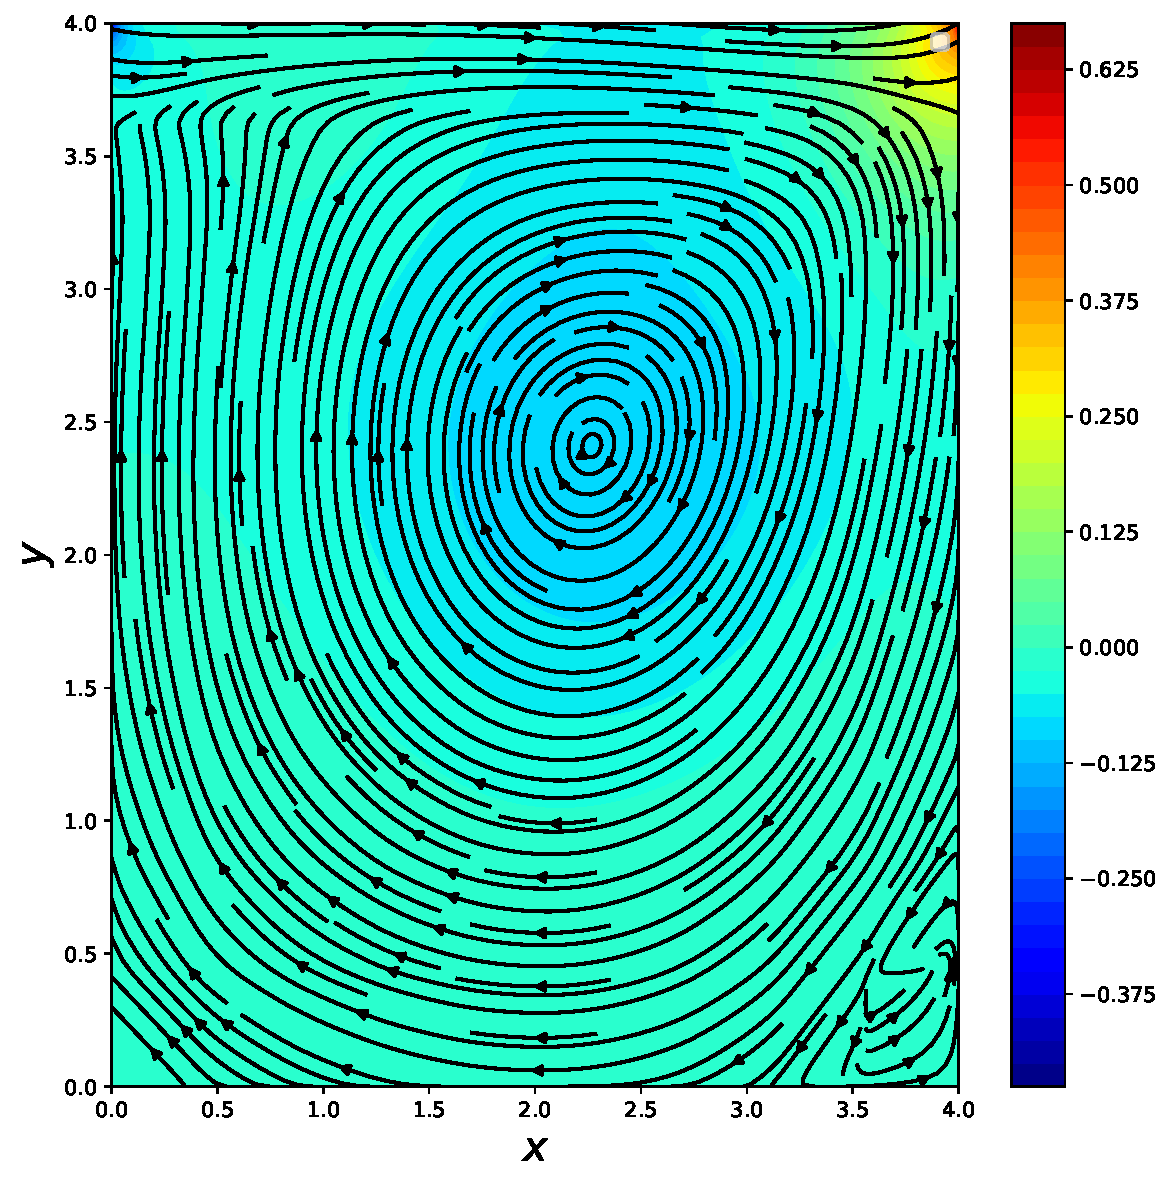
\includegraphics[width=\linewidth]{./images/Re400FlowPy_pres_stream}
%		\caption{Streamlines ($\psi$)}
%		\label{fig:pres_example1}
%		\endminipage\hfill
%		\minipage{0.32\textwidth}
%		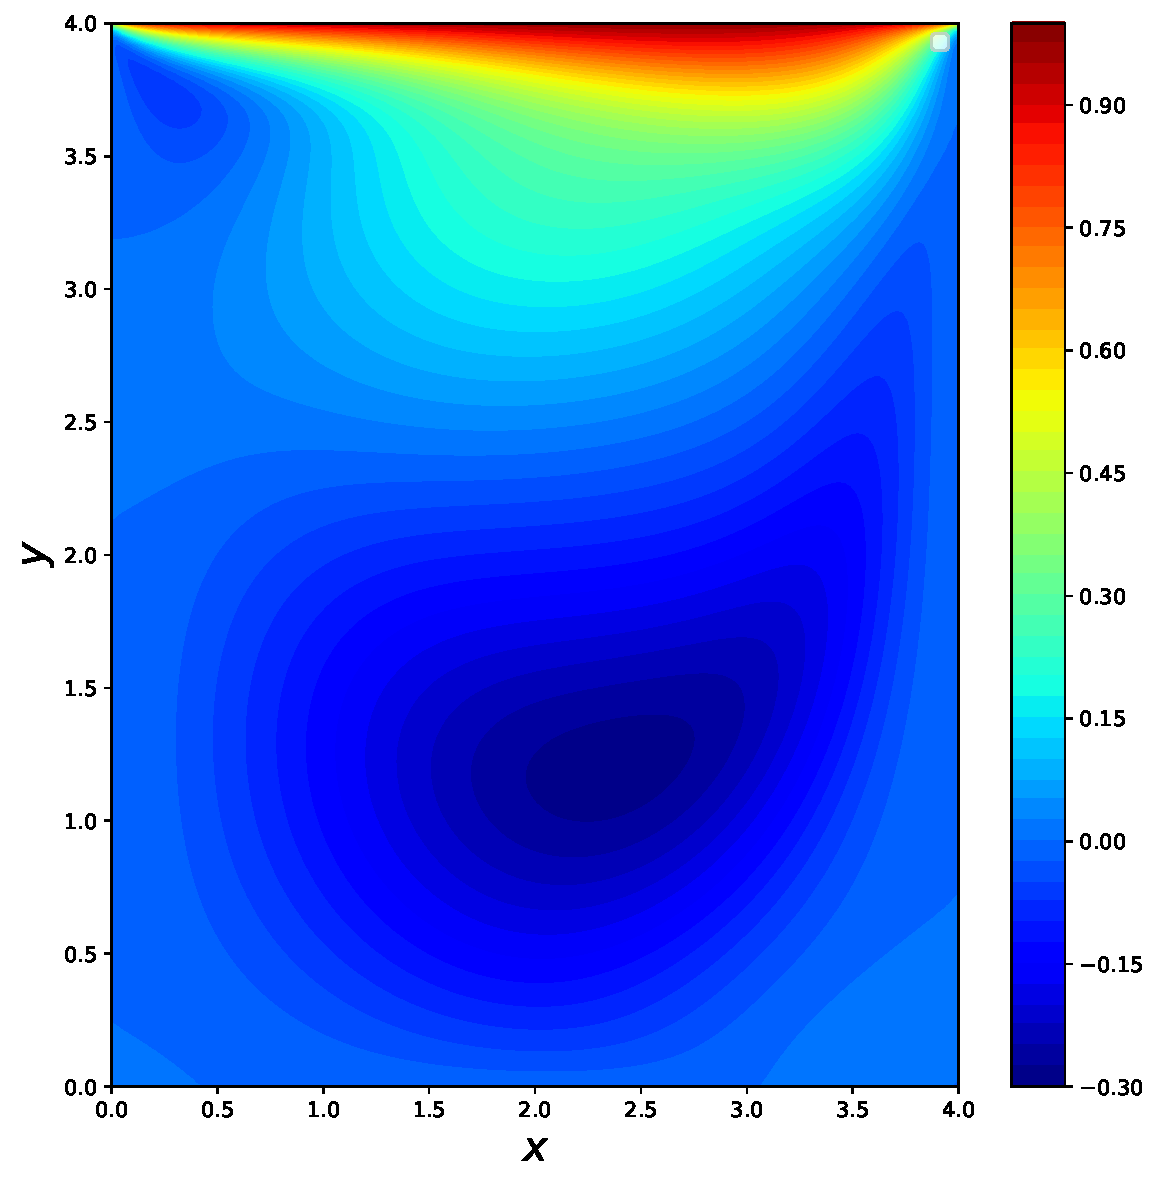
\includegraphics[width=\linewidth]{./images/Re400FlowPy_u}
%		\caption{U Velocity $Re = 400$}
%		\label{fig:u_example1}
%		\endminipage\hfill
%		\minipage{0.32\textwidth}%
%		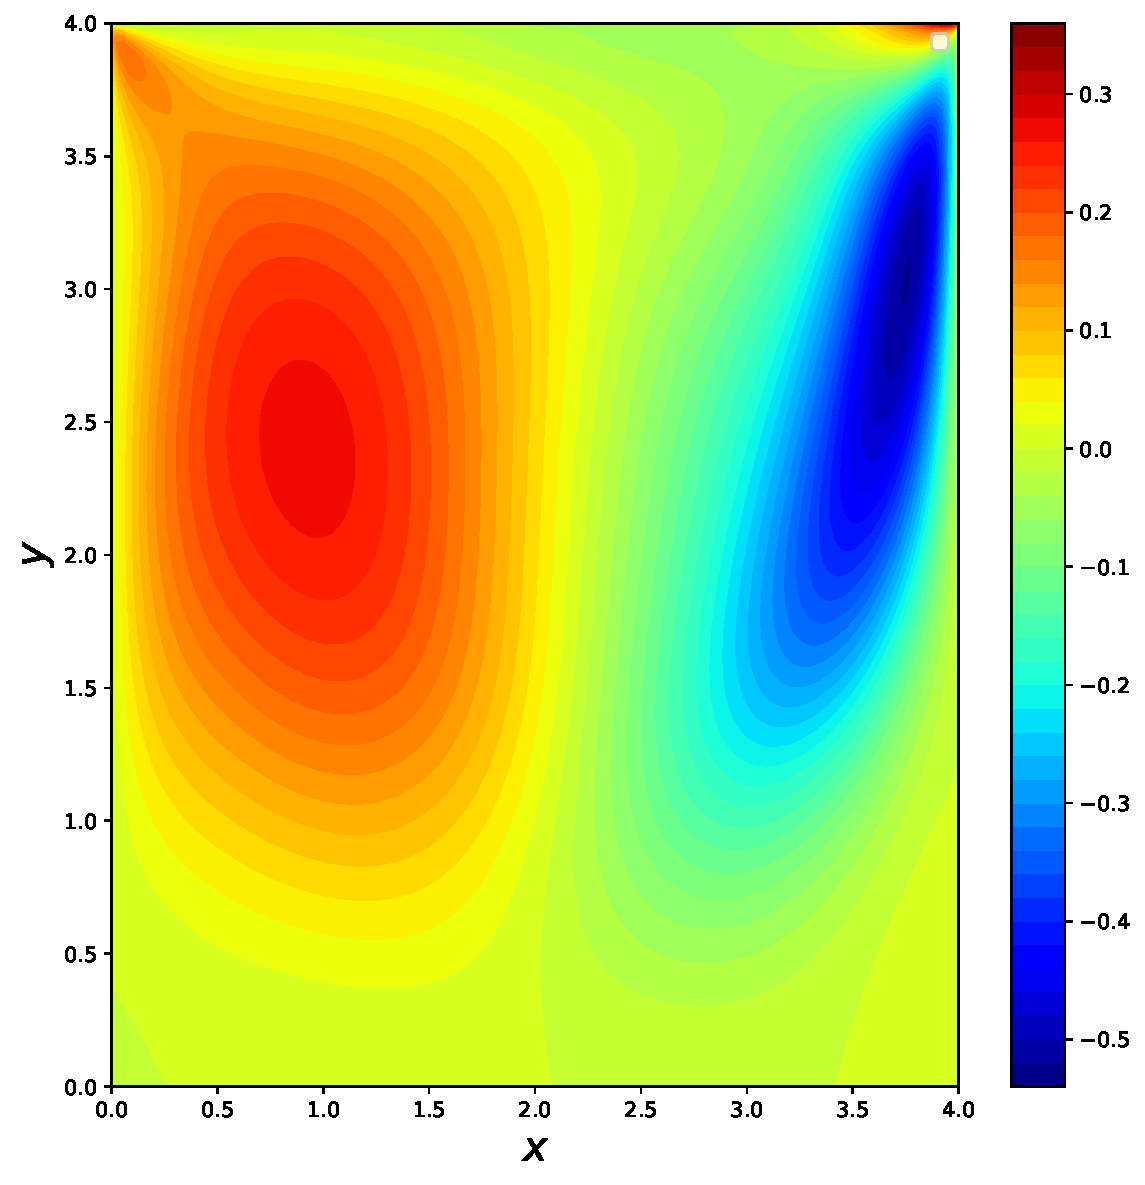
\includegraphics[width=\linewidth]{./images/Re400FlowPy_pres_v}
%		\caption{V Velocity $Re = 400$}
%		\label{fig:v_example1}
%		\endminipage
%	\end{figure}
%	
%	\begin{figure}[htb!]
%		\minipage{0.32\textwidth}
%		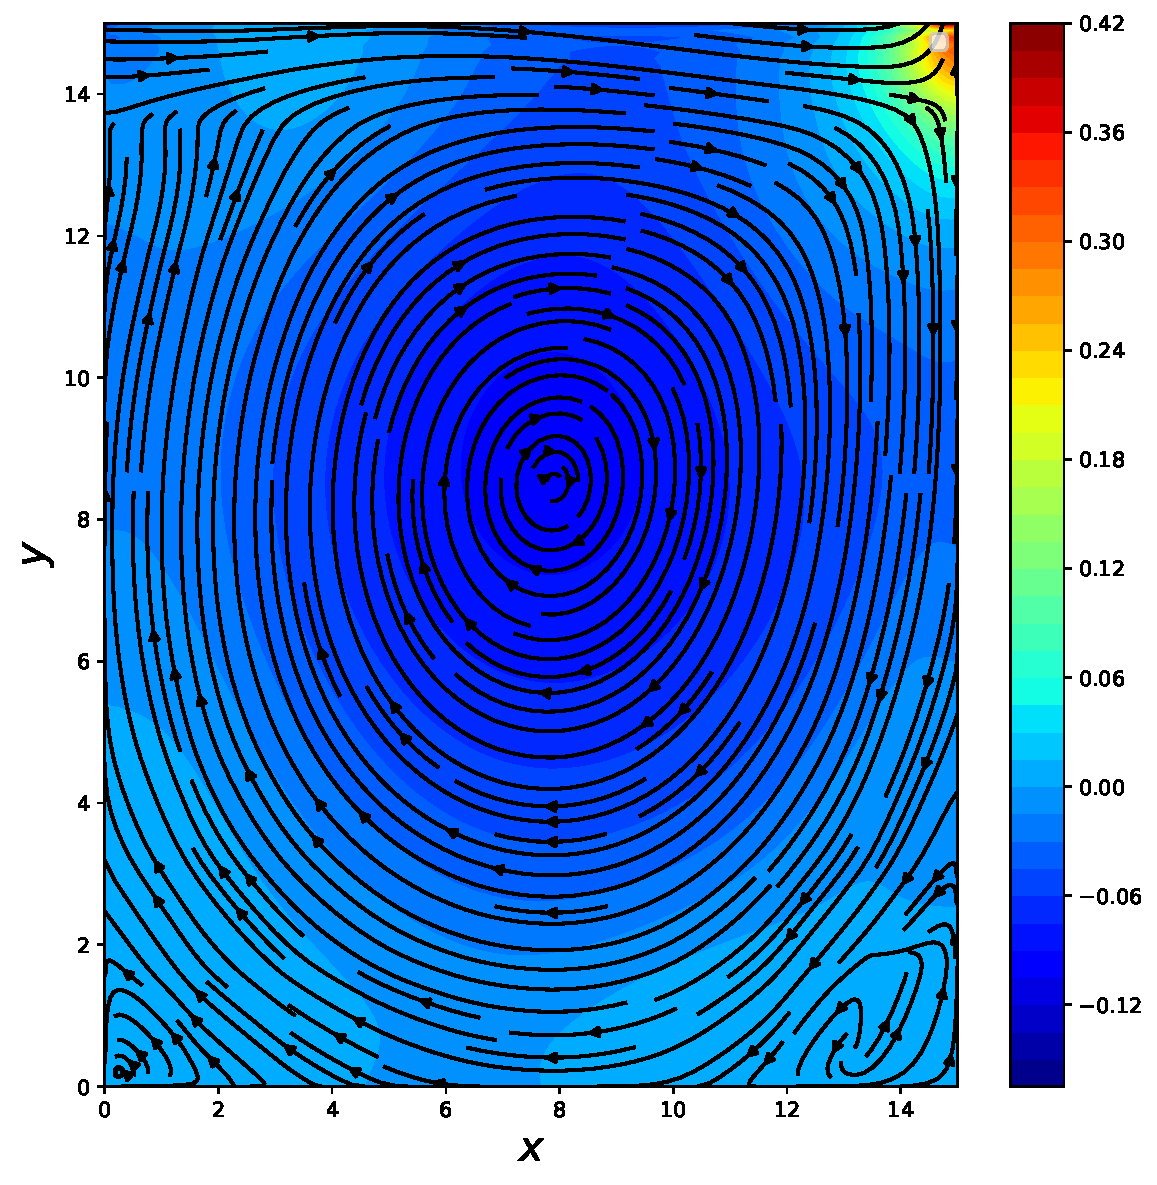
\includegraphics[width=\linewidth]{./images/Re1500FlowPy_pres_stream}
%		\caption{Streamlines ($\psi$)}
%		\label{fig:pres_example2}
%		\endminipage\hfill
%		\minipage{0.32\textwidth}
%		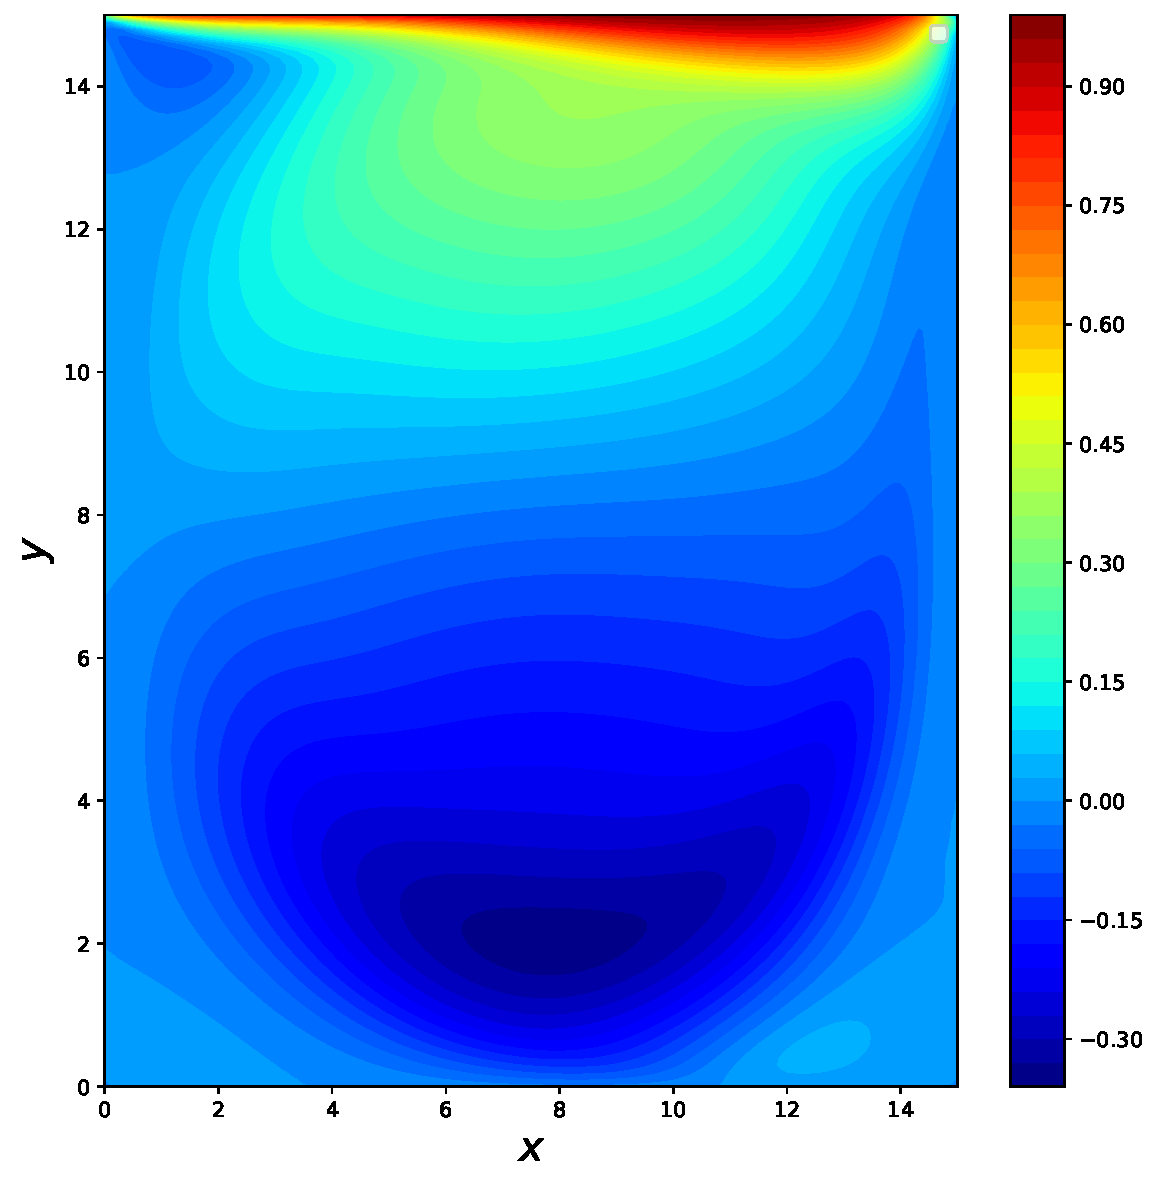
\includegraphics[width=\linewidth]{./images/Re1500FlowPy_u}
%		\caption{U Velocity $Re = 1500$}
%		\label{fig:u_example2}
%		\endminipage\hfill
%		\minipage{0.32\textwidth}%
%		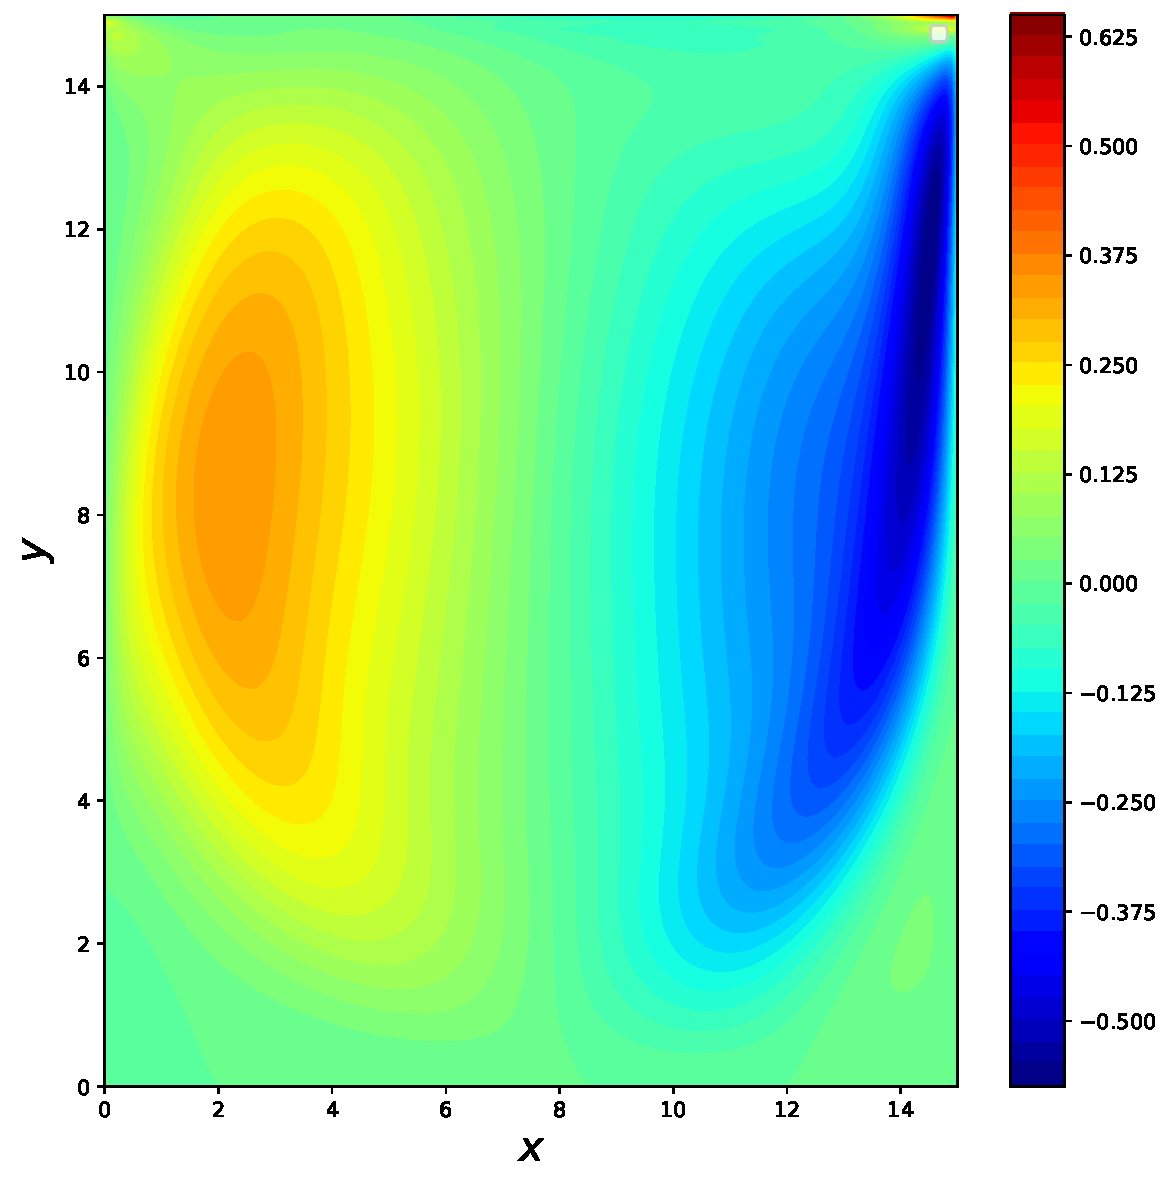
\includegraphics[width=\linewidth]{./images/Re1500FlowPy_pres_v}
%		\caption{V Velocity $Re = 1500$}
%		\label{fig:v_example2}
%		
%		\endminipage
%	\end{figure}
%	
%	Overall the FlowPy results converged nicely, and usually take 5-10 minutes to converge depending on how long in time the model is run. There are many observations of note that could help determine the validity of BoxFlowNet and the prediction results. For the predictions to keep the observations concise only the difference of the U velocity will be observed. The list below are the features most noteworthy:
%	
%	\begin{itemize}
%		\item Bottom left and right corners of \autoref{fig:pres_example1} and \autoref{fig:pres_example2} have smaller vortices, where the higher Reynolds number's bottom left corner is slightly more developed.
%		\item Lower speed zones (darkest blue regions) in \autoref{fig:u_example1} and  \autoref{fig:u_example2} move lower with respect to y the higher the speed of the fluid. This is due to a more energetic flow.
%		\item V velocity high and low speed regions on the left and right of \autoref{fig:v_example1} and \autoref{fig:v_example2} have different shapes and sizes.
%	\end{itemize} 	
%	
%	And now for the interesting part... or in this case, not so interesting! This was a great, really fascinating study, however it's very apparent that the model is either severely under-fit,
%	or the model needs convolution etc, to predict the spatial element. However it is worth nothing that the model isn't completely wrong, which leads me to conclude with the right layer tweaking this might be on to something. The reasoning behind this is the higher (or higher u velocity) is on the top, with a lower pressure on the bottom! A few things that come to mind with respect to what could be going on, is the resolution is simply too high, since the original code base for \citeauthor{DBLP:journals/corr/abs-1711-10566} used multiple optimizers, one being a specifically difficult to implement L-BFGS optimizer for the lambdas, and a regular Adam, while this model only used 2 parameter sets one with the weights and another with the lambdas. Another issue that might have caused this are the autograd calls to differentiation as seen in equation 12. Overall a very fun and interesting project, even if the model didn't fit very well and tweaking would be required. 
%	\begin{figure}[htb!]
%		\minipage{0.32\textwidth}
%		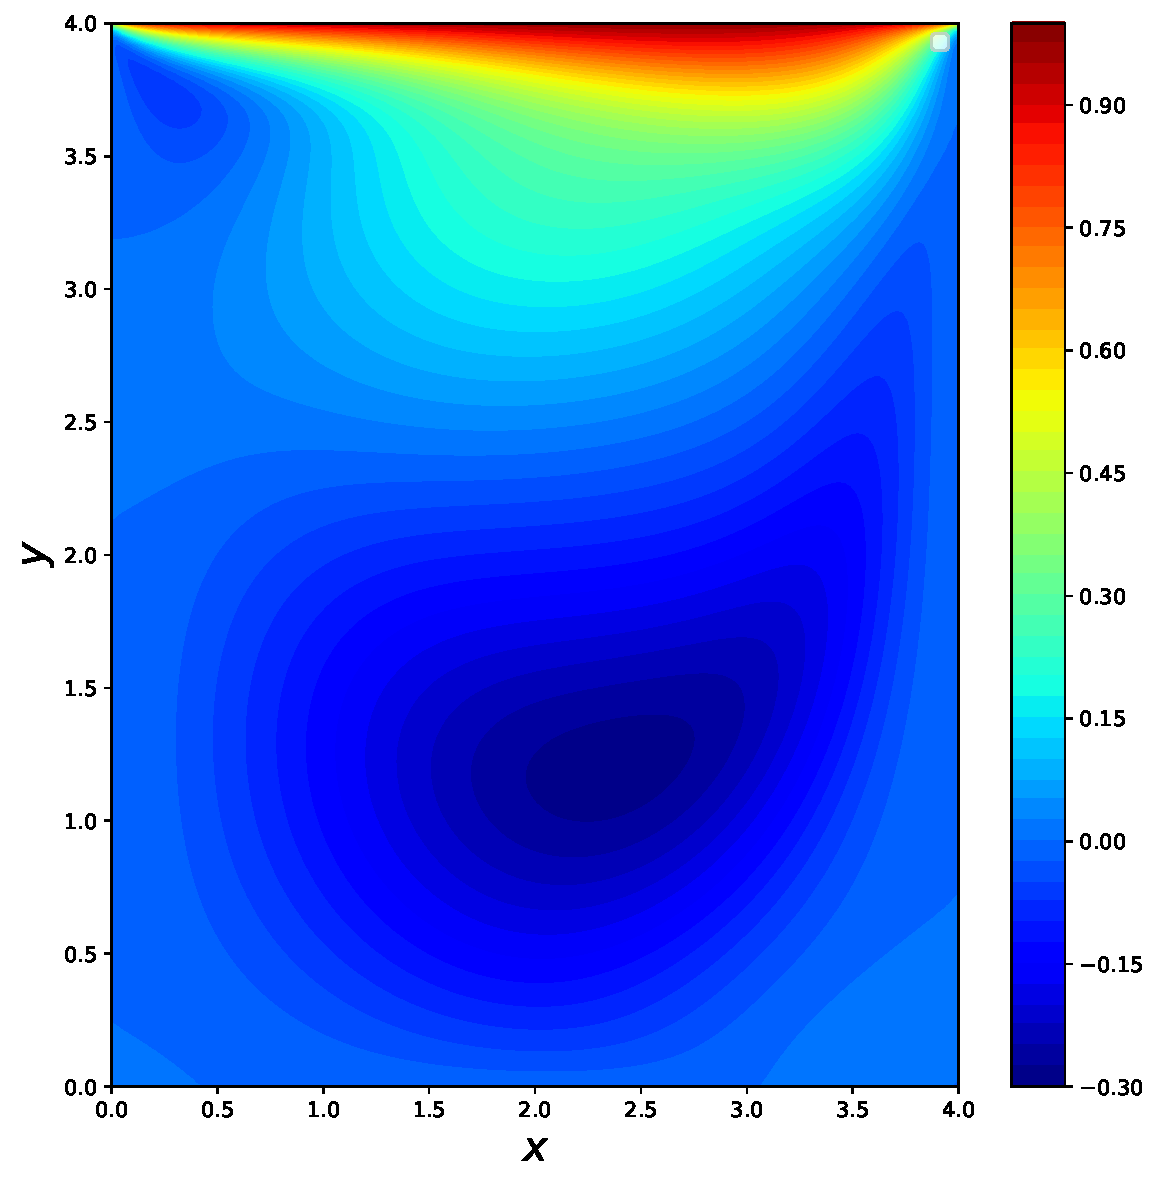
\includegraphics[width=\linewidth]{./images/Re400FlowPy_u}
%		\caption{Original U (FlowPy)}
%		\label{fig:u_oigin}
%		\endminipage\hfill
%		\minipage{0.32\textwidth}
%		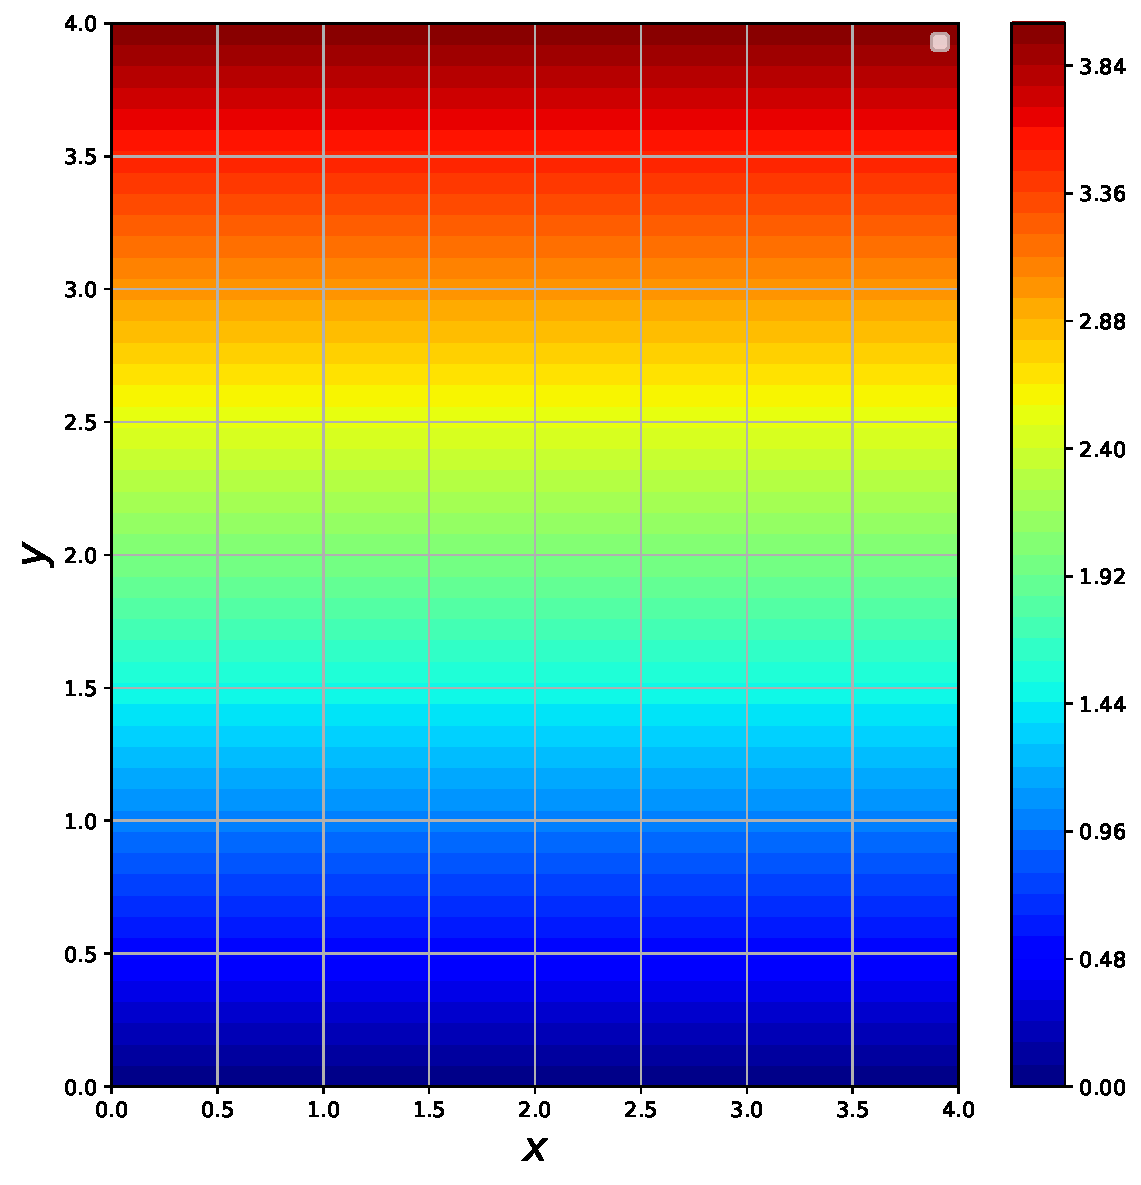
\includegraphics[width=\linewidth]{./images/Re400BoxFlowNet_pred_u}
%		\caption{predicted U at $Re = 400$}
%		\label{fig:u_pred}
%		\endminipage\hfill
%		\minipage{0.32\textwidth}%
%		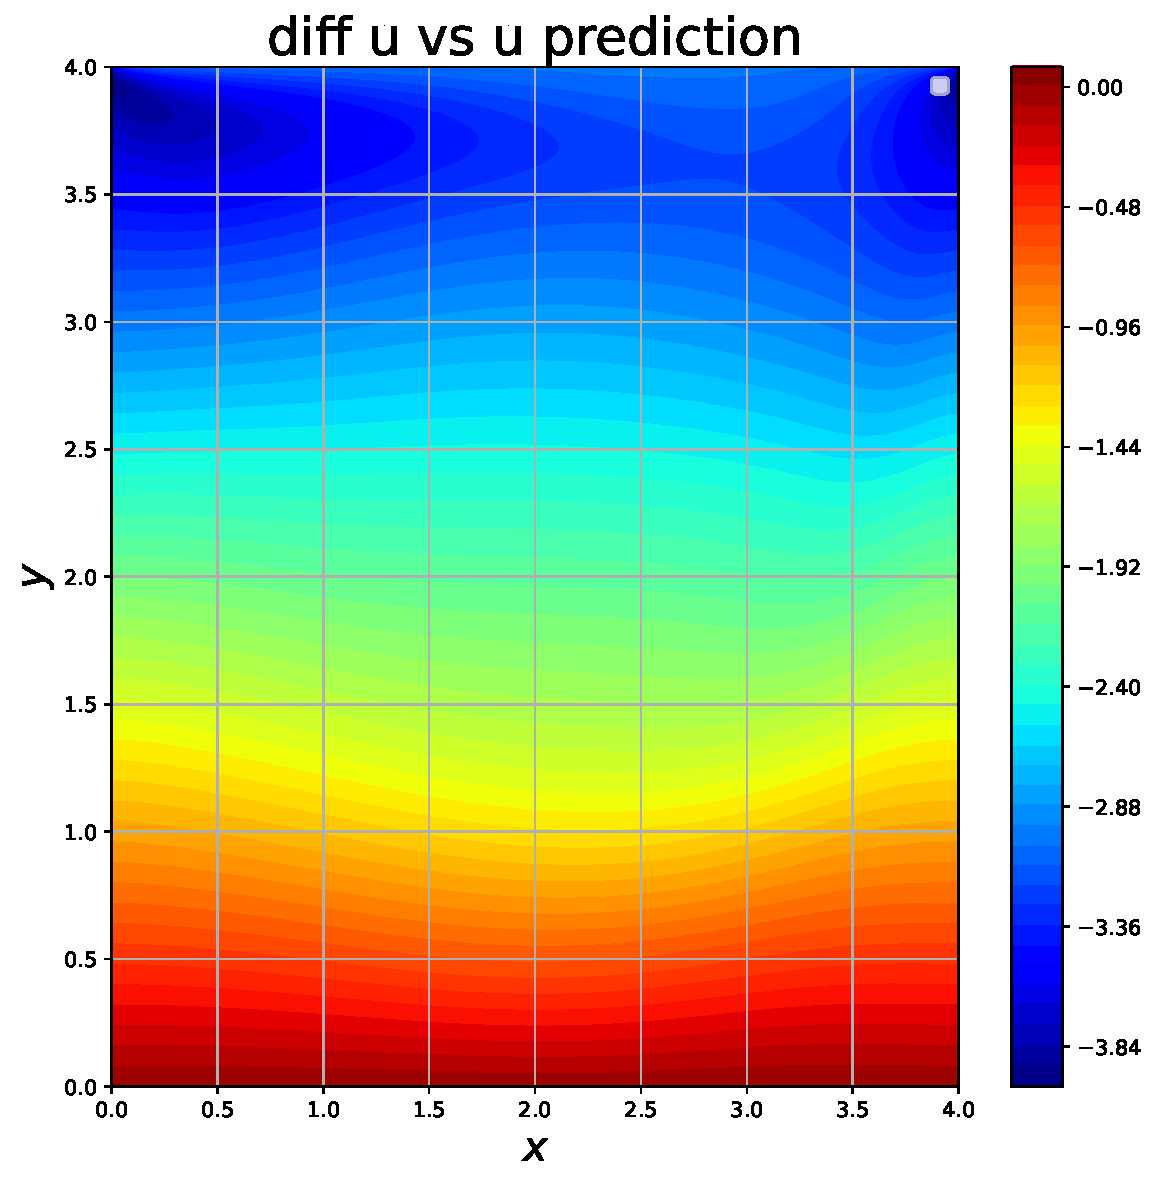
\includegraphics[width=\linewidth]{./images/Re400BoxFlowNet_diff_u}
%		\caption{U minus U predicted}
%		\label{fig:u_diff}\hfill
%		
%		\endminipage
%	\end{figure}
%	
%	\begin{figure}[htb!]
%		\centering
%		\includegraphics[scale=0.5]{./images/Re400BoxFlowNet_pres}
%		\caption{"pressure" (i.e. model weights)}\label{fig:pred_pres}
%		\label{fig:SIMPLE_pres2}
%	\end{figure}
%	
	%	\begin{equation}
		%	\begin{aligned}
			%		a_t &= Ux_t + W h_{t-1} + b \\
			%		h_t &= \tanh(a_t) \\
			%		o_t &= Vh_t + c \\
			%		\hat{y}_t &= \text{softmax}(o_t) \\
			%		L_t &= \text{CE}(\hat{y}_t, y_t)
			%	\end{aligned}
		%	\end{equation}
	%	
	%	\begin{equation}
		%	\begin{aligned}
			%	\frac{\partial L_t}{\partial U} &= \frac{\partial L_t}{\partial \hat{y}_t} \frac{\partial \hat{y}_t}{\partial o_t} \frac{\partial o_t}{\partial h_t} \frac{\partial h_t}{\partial a_t} \frac{\partial a_t}{\partial U} \\
			%	&= (\hat{y}_t- y_t) \frac{\partial \hat{y}_t}{\partial o_t} V \frac{\partial h_t}{\partial a_t} \frac{\partial a_t}{\partial U} \\
			%	&= (\hat{y}_t - y_t) \frac{\partial \hat{y}_t}{\partial o_t} V \frac{\partial \tanh(a_t)}{\partial a_t} \frac{\partial a_t}{\partial U} \\
			%	&= (\hat{y}_t - y_t) \frac{\partial \hat{y}_t}{\partial o_t} V \text{sech}^2(a_t) \frac{\partial a_t}{\partial U} \\
			%	&= (\hat{y}_t - y_t) \frac{\partial \hat{y}_t}{\partial o_t} V \text{sech}^2(a_t) (x_t + h_{t-1})
			%	\end{aligned}
		%	\end{equation}
	
%	Code can be found here: https://github.gatech.edu/abartels3/Lid-Driven-Cavity-Flow-PINN
	
	%	We have:
	%	
	%	at = Uxt + Wht-1+b
	%	
	%	ht = tanh(at)
	%	Of = Vht + c
	%	yt = Softmax(of)
	%	Lt = CE(yt, yt)
	%	
	%	We want to compute:
	%	
	%	dU = dL/dU
	%	dW = dL/dW
	%	db = dL/db
	%	dc = dL/dc
	%	dV = dL/dV
	%	
	%	Using the chain rule, we have:
	%	
	%	dL/dU = dL/dOf * dOf/dht * dht/dat * dat/dU
	%	dL/dW = dL/dOf * dOf/dht * dht/dat * dat/dW
	%	dL/db = dL/dat * dat/db
	%	dL/dc = dL/dOf * dOf/dc
	%	dL/dV = dL/dOf * dOf/dht * dht/dat * dat/dV
	%	
	%	We can compute each of these derivatives as follows:
	%	
	%	dL/dOf = olt
	%	
	%	dOf/dht = V
	%	
	%	dht/dat = f'(at)
	%	
	%	dat/dU = xt
	%	
	%	dat/dW = ht-1
	%	
	%	dat/db = 1
	%	
	%	dat/dV = ht
	%	
	%	dat/dc = 1
	%	
	%	Putting it all together, we have:
	%	
	%	dU = olt * V * f'(at) * xt
	%	
	%	dW = olt * V * f'(at) * ht-1
	%	
	%	db = olt * V * f'(at) * 1
	%	
	%	dc = olt * V * 1
	%	
	%	dV = olt * ht
	%	
	%	This is how we compute the gradients for a 4 length RNN.
	%	
	%	Assuming a 4 length sequence RNN, we can compute the derivative of the Loss function with respect to the output of the RNN as follows:
	%	
	%	dL/dOf = dL/d Lt * dLt/dOf
	%	
	%	= (yt - yt) * Vht
	%	
	%	= yt*Vht - yt*Vht
	%	
	%	= yt*(Vht - Vht)
	%	
	%	= 0
	%	
	%	Therefore, the derivative of the Loss function with respect to the output of the RNN is 0.
	%	
	%	Similarly, we can compute the derivative of the Loss function with respect to the hidden state of the RNN as follows:
	%	
	%	dL/dht = dL/d Lt * dLt/dht
	%	
	%	= (yt - yt) * Vht * dOf/dht
	%	
	%	= (yt - yt) * Vht * Vht-1 * f'(ht-1)
	%	
	%	= (yt - yt) * Vht * Vht-1 * (1 - f(ht-1)\^2)
	%	
	%	= (yt - yt) * Vht * Vht-1 * (1 - ht-1\^2)
	%	
	%	= yt*Vht*Vht-1*(1-ht-1\^2) - yt*Vht*Vht-1*(1-ht-1\^2)
	%	
	%	= yt*Vht*Vht-1 - yt*Vht*Vht-1
	%	
	%	= 0
	%	
	%	Therefore, the derivative of the Loss function with respect to the hidden state of the RNN is also 0.
	%	
	\clearpage
	
	\printbibliography
	
	
\end{document}

